
\section{Limitations \& Future Work}\label{section:lim}

Our project leveraged Unity and Processing to build a proof-of-concept WVC system. We investigated machine-learning-based gaze-tracking technologies and real-time avatar rendering. We also implemented our own WVC system and we successfully integrate it with gaze-tracking technology. But we realized that it is very time consuming to achieving real-time avatar rendering, especially considering this is a course project. We decided to build mock meeting scenes and implemented pre-programmed avatars in Unity to avoid spending time on achieving real-time rendering. The main goal of the paper is to explore the impact and usefulness of eye-contact in WVC system rather than making a working product.

The major limitation is that the avatar may not be as realistic as the human face. So, talking to an animated head with fake eyes may not give the participants the same eye contact experience as in real life. The number of participants in the meeting is another drawback of this prototype; if there are more than 15 participants, their avatars would be arranged into more than one page. While we can overcome the arrangement issue trivially by programming a custom front-end, each participant will have a tiny grid, making the gaze-tracking component a challenge. 

5 participants (P4, P6,  P10, P8, P11) mentioned details on pupils that can be further improved. As P10 described,  ``\textit{typically heads do not move as much during traditional online meeting apps and once someone else is speaking, eyes will shift rather than heads.}" P8 also thinks that our head model does not reflect the real life situation good enough because there are no pupils in the head. P8 said ``\textit{I think it is a good idea to represent people with fake heads, but their eyes did not have a pupil so it was hard for me to tell who is looking at whom based on the eye movement.}" P6 agreed with P10 and mentioned head models without pupils is unnatural for them to look at. Additionally, P4 noted that our eye model is not very realistic since the eyeballs in real life will not be fixed when people are paying attention; people turn their heads and keep blinking their eyes rather than having their eyes fixed. P11 also indicated that ``\textit{The eyes of the avatars could be detailed and optimised for better attention catching for the audiences.}"

After all experiments, we asked participants for their feedback and suggestions for improving our system. Most participants complimented our system and one participant said ``\textit{It's nice enough for me to use it.}" There are two most common suggestions we gathered from the participants. First, improving the rendering quality of the avatars (P4, 7, 8, 9, 10, 11). P4 mentioned \textit{``Obviously, if the avatars are more vivid, and they do represent your eye contact, your direction of looking, maybe even body gesture etc, it could be significantly improving how it is, and avoiding the nervousness and awkwardness with real images." }However, the trade-offs of implementing more realistic avatars need to be considered carefully. P8 thinks the current head model in our system is less realistic, \textit{ ``I think the talking head version is somehow less realistic than the eyes version. Maybe it was because the head is trying to be more realistic, but it is still different from how a real head looks, so it breaks immersion for me."} With more realistic avatars, uncanny valley phenomena might arise. When the head model is closer to the realness but some tiny differences still exist, people tend to feel very comfortable. It also has the risk of breaking the immersion. 

Second, adding more functionalities to the avatar (P2, 4, 10, 12), such as body gesture (P4), head nodding (P2), mouth animation(P10), and customization of avatars (P10) would make our system even better. Two participants (P1, 12) mentioned they’d like to see more features for our system. For example P1 commented ``\textit{give option to switch between 2d and 3d}". P6 thinks our system makes people feel more interactive. They stated that `` \textit{I'd like to see that the avatars could reflect some states of the people who are participating in a virtual conference. This will truly make people feel more interacted.}" 

Overall, the project documented in this report is only a single component of the entire stack
that is required to create a fully-functional app. 
Other key components that is not mentioned here (since they are not relevant to the research question) include
networking using web sockets, computer graphic optimizations, encryption and security, privacy, data transmission,
gaze tracking, etc.
Figure \ref{fig:dataflow} shows the proposed data flow and modules of a completed FutureGazer app.

\begin{figure}
	\centering
 	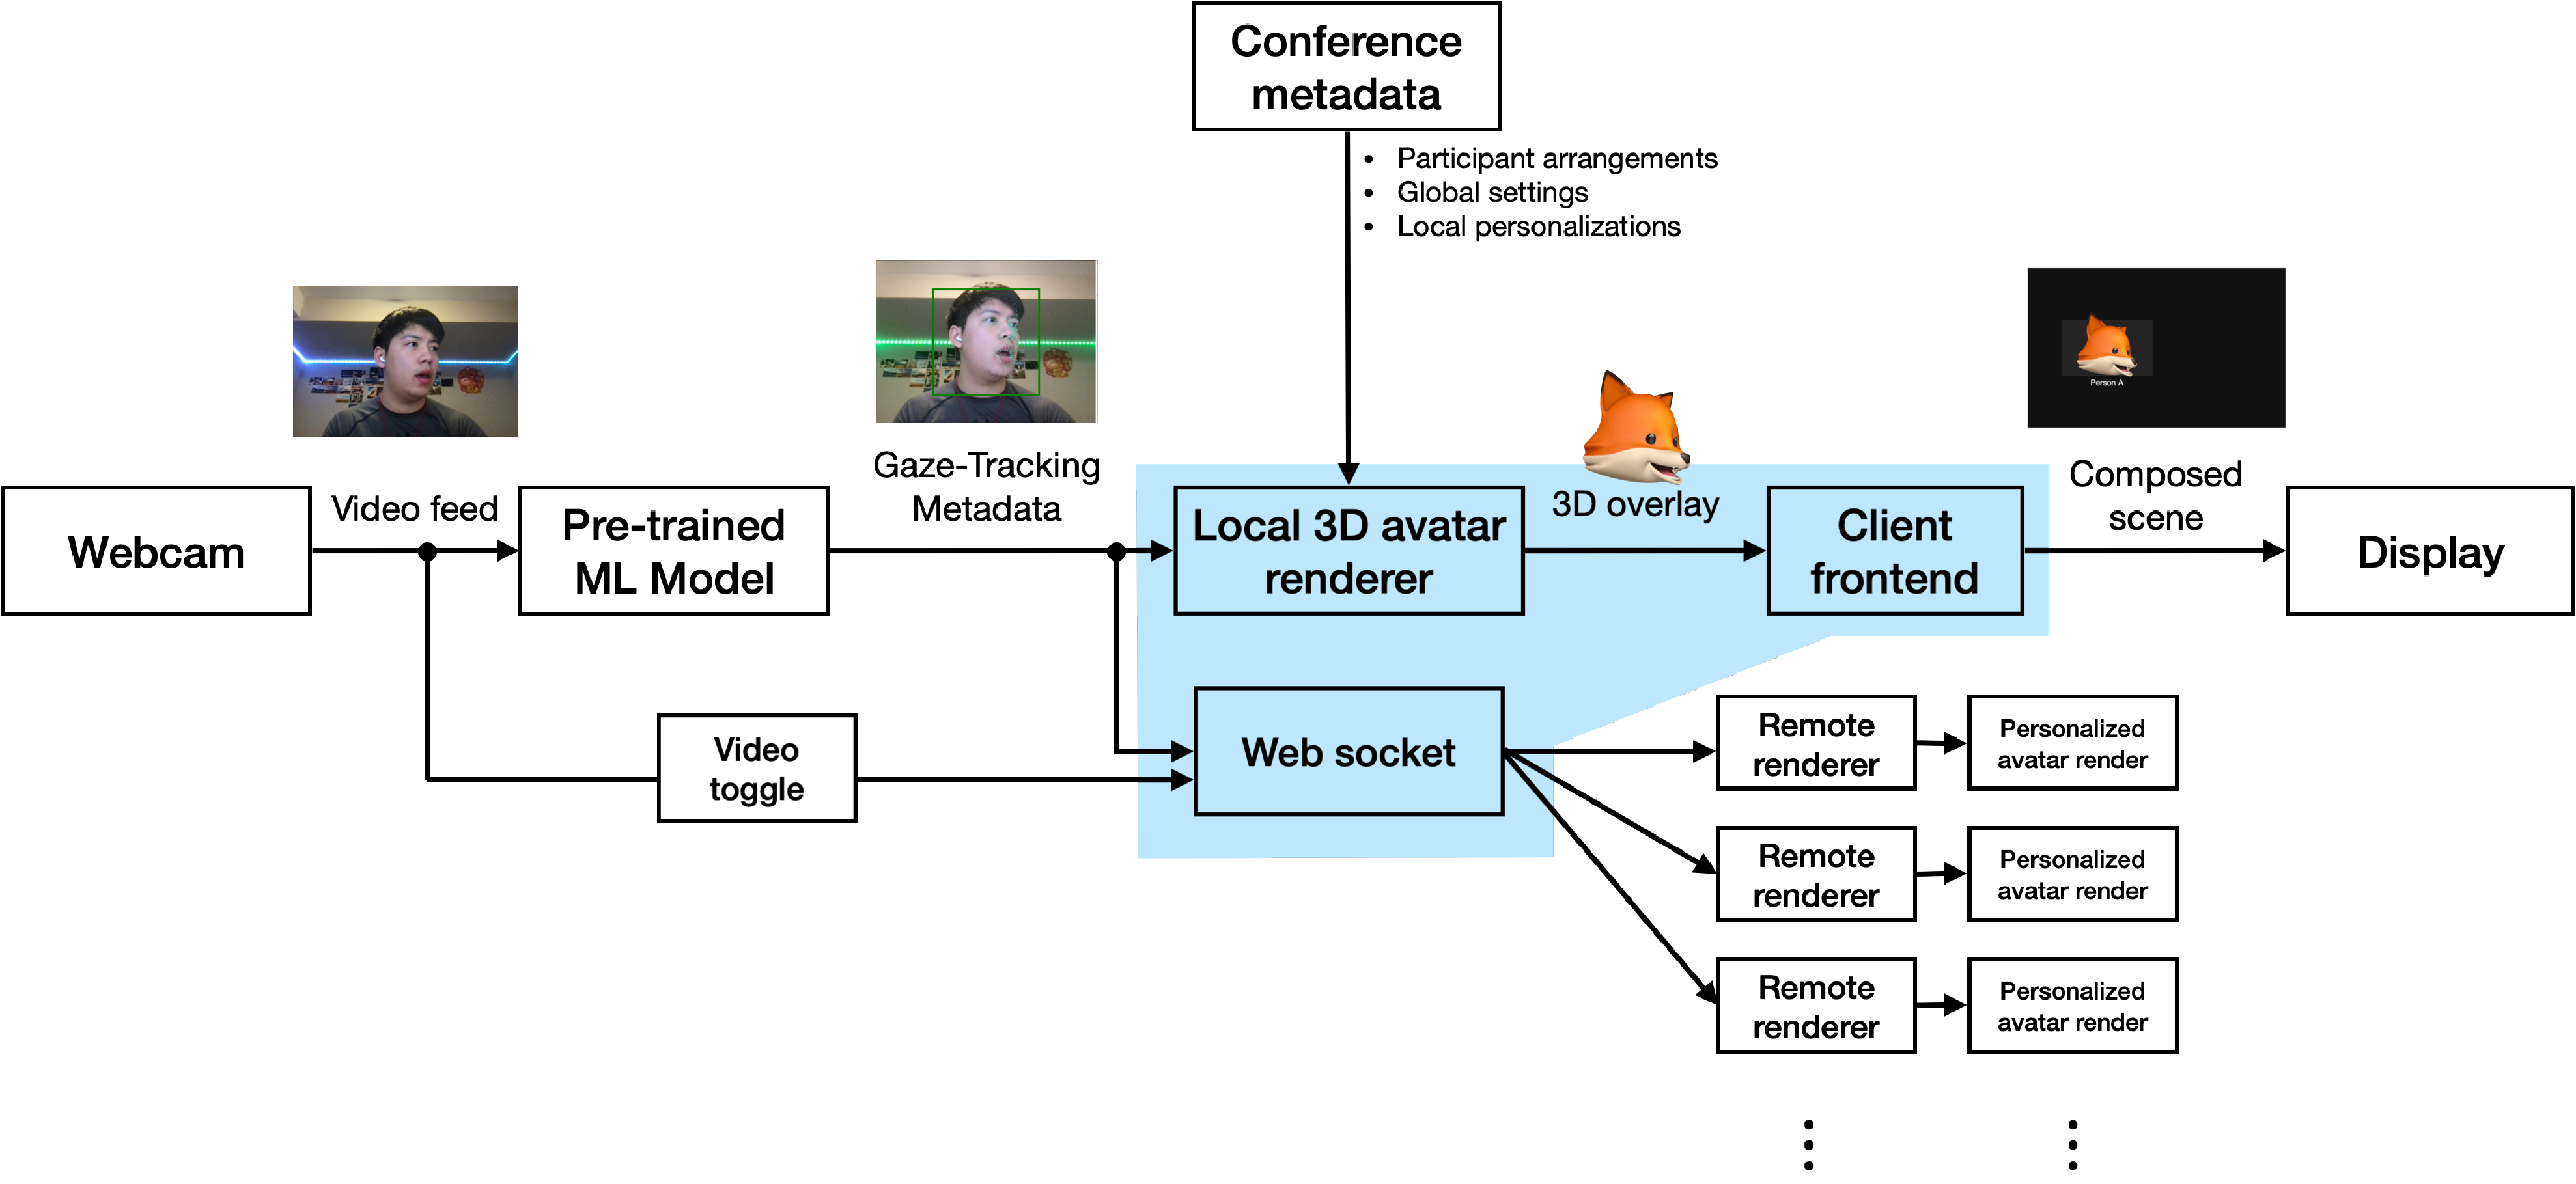
\includegraphics[width=\textwidth]{dataflow.pdf}
	\caption{Data flow and block diagram of an ideal fully-functional FutureGazer WVC application}
	\label{fig:dataflow}
\end{figure}

% - Covid-19 working remotely, so it’s hard to sync up between team members
% - Technical limitations (technical)
% 	- 2D and 3D avatars/views are primitive (barely colours and textures)
% 	- Not customizable, could affect how people feel about usability because it doesn’t convey as much expression as originally intended
% 	- 3D head lack eyes with animation and texture (unfinished due to technical and time constraints) -- also affects how people perceive eye-contact in WVC because it looks creepy (and literally have no eyes).
% 	- Primitive lighting in 3D environment (simple directional light creates uncanny environment)
% - Limitations in running the experiments:
% 	- User testing extremely difficult, despite the prototype framework being cross-platform, exporting/deploying apps required notarization (a security feature that only allows officially signed app to run), so we need last-minute hacks to have the user experiments run
% 	- Small sample size
% - Limitations in collection of data
% 	- Ideally, we want to use some gaze-tracking hardware/software to actually track and log where the users are looking at (as seen in the omitted experiment setup using Tobii), but because none of the user experiments are performed in person, we physically cannot collect those data.
% 	- A workaround is to have the user click/move the mouse to where they’re looking at, but because of aforementioned platform limitations, we can’t do that either
% - Bias of data
% 	- Sample size could be to homogeneous (break down of first-spoken language, ethnicity, geographic location)
% 	- Time of day when running the experiment affects participant’s attention, energy, and mood, and ultimately affect experiment outcomes

% \subsection{Prototype Development}

% - Unified 3D framework/engine
% - Apple Gatekeeper notarization 
% - More sophisticated 3D models and animations
% - Add real-time gaze tracking support
% - More dynamic and fluid 3D environment (since right now all the heads and eyes are locked onto a grid)
% - 